\section{Methodology}

\subsection{MinHash and Locality-Sensitive Hash Forest}

In order to reduce packet data to a set intersection problem, contents must first be \textit{shingled} into items which will make up the set. An object is $w$-shingled when a sub-sequence of length $w$ of contiguous tokens is cut from it. In \textsc{Alpine}, we use the port information, transport layer protocol, flag values, and packet length to make up our shingles. In \textsc{Palm}, word tokens are created by delimiting packet payloads by whitespace. Thus, each original packet $P$ is now associated with some set $S_P$ of shingles as depicted in Figure~\ref{jacsim}.

\begin{figure} [ht!]
\begin{equation}
J(P_A, P_B) = \frac{|S_A \cap S_B|}{|S_A \cup S_B|}
\end{equation}
\caption{Jaccard Similarity of Shingle Sets}
\label{jacsim}
\end{figure}

MinHash may be used to quickly approximate the Jaccard similarity between two sets. The hash signatures take up a fixed and smaller amount of space than large shingle sets and can be used to normalize the data in cases where the shingle set features are of varying lengths and types. The MinHash of a given column is the number of the first row in permuted order whose characteristic matrix value is $1$. This sequence is continued down the columns and repeated for $k$ permutations. The probability that the MinHash function for a random permutation of rows produces the same value for two sets is a close approximation to their Jaccard similarity~\cite{mmds}. We use the LSHForest algorithm developed by Bawa et al~\cite{lshforest} to index the locality-sensitive hashes and optimize the search process. It improves upon nearest-neighbor searches by both reducing complexity and eliminating the need to know the distance $r$ from the query to the nearest neighbor of a given data point. This optimization is achieved through the use of a specific set of hash functions which ensures that any nearest neighbor query returns $\epsilon$-approximate neighbors so long as a suitable $l$ number of trees is chosen. Compared to previous work which uses nearest neighbor searches~\cite{fpga}, LSHForest scales much more efficiently. The build time of a KNN model can have a complexity of $O(n^2)$, where $n$ is the number of items. In contrast, LSH construction is done in linear time~\cite{lshforest}. The theoretical complexities of operations on LSHForest are provided from the original paper in Table~\ref{table:forestcomplex}. When compared with time and space complexities for the automata in regular expression searching in Table~\ref{table:facomplex}, the logarithmic improvement and fixed storage space is clear.

\begin{table} [ht!]
\caption{Time Complexities for LSHForest~\cite{lshforest}}
\centering
\begin{tabular}{|c | c |}
\hline
\textbf{Operation} & \textbf{Complexity} \\
\hline
Insertion & $O(l * log_B n)$ \\
\hline
Deletion & $O(l * log_B n)$ \\
\hline
Query &  $O(l * log_B n) + O(l * log B) + O(M/B)$\\
\hline
\end{tabular}
\label{table:forestcomplex}
\end{table}

In these equations, $l$ represents the number of trees, $B$ the branching factor of an internal node, and $n$ the number of data points in the dataset. Storage is also optimized to be linear, $O(n)$, through the use of compressed PATRICIA tries~\cite{lshforest}. The query for some point $q$ for $m$ nearest neighbors first performs a binary search for the longest matching prefix at a leaf node with the point $s_i$. Then some $M$ points are collected synchronously across all trees and ranked by similarity score, with the top $m$ being returned as an answer. We use the $m$ number as votes to ultimately classify the sample by majority once the query is performed. This majority vote approach also allows for multiple classification results; for example, an adaptive system may be able to take the second closest result if the first choice turns out to be erroneous.

\subsection{ALPINE: A Locality-Based Packet Inspection Engine}
\textsc{Alpine}~\cite{alpinepalm} is \textbf{A} \textbf{L}ocality-Sensitive \textbf{P}acket \textbf{In}spection \textbf{E}ngine which performs shallow packet inspection on selected features from the network and transport layer encapsulation headers of packets. \textsc{Alpine} uses Jaccard similarity in order to determine likeness between sets of the following packet header features: \textit{source and destination IP address, type of service field, packet length, IP next protocol, IP flags, source and destination port} (see Figure~\ref{fig:alpineheader}). For indexing the computed MinHashes and performing lookup for classification, \textsc{Alpine} uses the previously discussed LSHForest~\cite{lshforest}. A query is performed by computing the MinHash of the input data and doing a binary search on the prefix trees. The hash is then mapped back to its label index. A majority vote is taken from the returned $m$ nearest neighbors and the data is classified accordingly.

\begin{figure} [ht!]
  \centering
  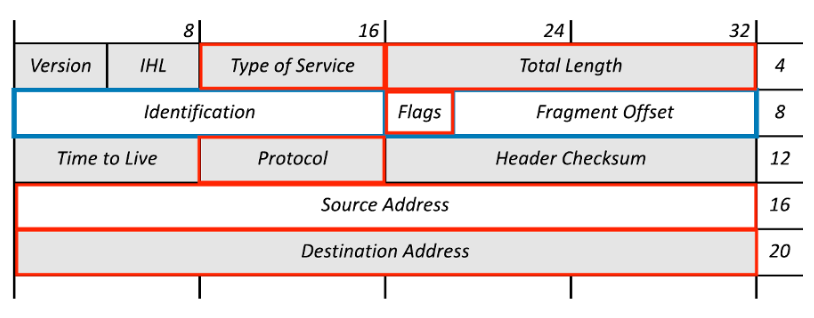
\includegraphics[width=0.8\textwidth]{chapters/4/img/alpineheader.png}
  \caption{Example TCP/IPv4 header with extracted features for \textsc{Alpine} highlighted in red.}
  \label{fig:alpineheader}
\end{figure}

\subsection{PALM: Payload Analysis Using Locality Sensitive Measurements}
\textsc{Palm} performs \textbf{P}ayload \textbf{A}nalysis using \textbf{L}ocality-Sensitive \textbf{M}easurements. This is a similar strategy to previous work in payload signature generation like SigBox~\cite{sigbox} and RExACtor~\cite{rexactor}. \textsc{Palm} delimits packet payloads by whitespace in order to create word-style tokens. In future work, other delimiters or a sliding-window shingling technique may suit identification of certain data types such as binary application layer protocols like HTTP2. In the experiments presented in this report, whitespace proved to be the most effective delimiter. We also experiment without using port numbers as identifiers in order to test the possiblity of non-standard port usage and detection. MinHash was used to generate the locality-sensitive hashes for the data samples and test samples. We use the LSHForest algorithm developed by Bawa et al~\cite{lshforest} to index the locality-sensitive hashes and optimize the search process.
